\documentclass[tikz, border=1mm]{standalone}
\usepackage{tikz}
\usetikzlibrary{shapes,arrows,calc,automata}
\begin{document}
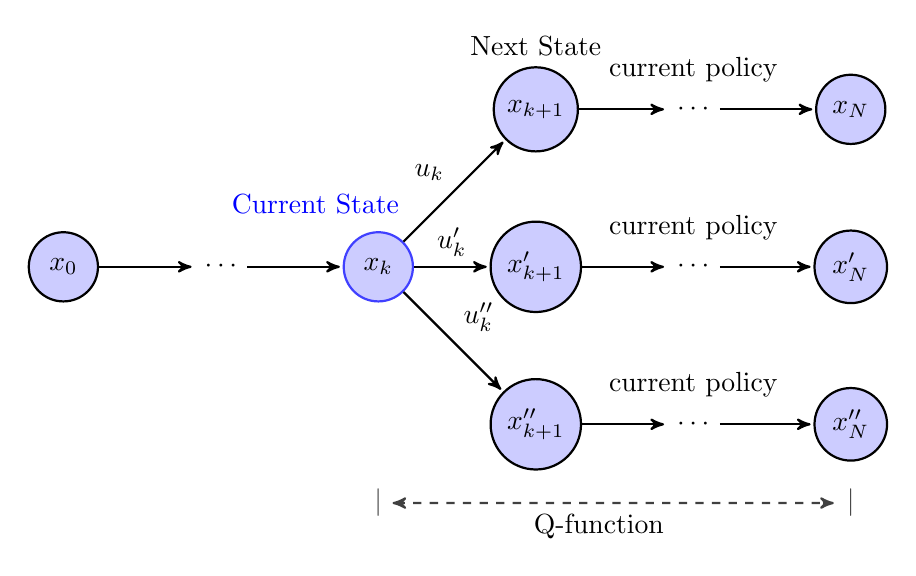
\begin{tikzpicture}[->,>=stealth',shorten >=1pt,auto,node distance=2cm, thick]
  \tikzstyle{every state}=[draw=black,fill=blue!20,text=black]
  \tikzstyle{dots}=[thick,draw=none,fill=none,text=black]
  \tikzstyle{place}=[draw=none,fill=none,text=black!75]
  \tikzstyle{texto}=[draw=none,fill=none,text=black]
  \node[state] (A)              {$x_0$};
  \node[dots ] (B) [right of=A] {$\cdots$};
  \node[state,draw=blue!75] (C) [right of=B] {$x_{k}$};
  \node[state] (D) [right of=C] {$x'_{k+1}$};
  \node[state] (E) [above of=D] {$x_{k+1}$};
  \node[state] (F) [below of=D] {$x''_{k+1}$};
  \node[dots] (D1) [right of=D] {$\cdots$};
  \node[dots] (E1) [right of=E] {$\cdots$};
  \node[dots] (F1) [right of=F] {$\cdots$};
  \node[state] (DN) [right of=D1] {$x'_N$};
  \node[state] (EN) [right of=E1] {$x_N$};
  \node[state] (FN) [right of=F1] {$x''_N$};
      \node[texto,text=black] (t1) [above of=D1,yshift=-1.5cm] {current policy};
      \node[texto,text=black] (t2) [above of=E1,yshift=-1.5cm] {current policy};
      \node[texto,text=black] (t3) [above of=F1,yshift=-1.5cm] {current policy};
  \node[texto,text=black] (t4) [below of=F,yshift=.7cm,xshift=.8cm] {Q-function};
      \node[place] (k) [below of=C, yshift=-1cm] {$|$};
      \node[place] (l) [below of=FN, yshift=1cm] {$|$};
      \node[texto,text=blue] (t5) [above of=C,yshift=-1.2cm,xshift=-0.8cm] {Current State};
      \node[texto,text=black] (t6) [above of=E,yshift=-1.2cm] {Next State};
  % \node[place] (k) [below of=C, yshift=1.5cm] {$|$};
  % \node[place] (l) [below of=D, yshift=1.5cm] {$|$};
  % \node[texto] (f) [above of=F, yshift=-1.5cm] {Terminal Cost $r_N$};
  % \node[texto,text=black!75] (t1) [below of=C, yshift=1cm, xshift=1.75cm] {Stage $k$};
  % \node[texto] (t2) [below of=C, yshift=2.2cm, xshift=1.75cm, text=blue] {Control $u_k$};

  \path (A) edge node {} (B)
        (B) edge node {} (C)
        (C) edge node {$u'_k$} (D)
        (C) edge node {$u_k$} (E)
        (C) edge node {$u''_k$} (F)
        (D) edge node {} (D1)
        (E) edge node {} (E1)
        (F) edge node {} (F1)
        (D1) edge node {} (DN)
        (E1) edge node {} (EN)
        (F1) edge node {} (FN);
      \draw [dashed,<->,draw=black!75] (k) -- (l);
  % \path (C) [draw=blue] edge node {} (D);
  % \draw [dashed,<->,draw=black!75] (k) -- (l);
\end{tikzpicture}
\end{document}
